\RequirePackage{silence}
\WarningFilter{biblatex}{Patching footnotes failed}
\documentclass[10pt, compress,british,xcolor={svgnames,dvipsnames,x11names},trans]{beamer}

\usepackage{babel}
\usepackage{csquotes}
\usepackage{comment}
\usepackage{tikzsymbols}

%%% mtheme customisations
\usetheme[progressbar=frametitle,block=fill]{m}
\setmonofont[Scale=0.92]{Fira Mono}
\AtBeginSubsection{
\metroset{color/background=dark}
\frame[plain,c]{
  \begin{center}
  \begin{minipage}{25em}
    \usebeamercolor[fg]{section title}
    \usebeamerfont{section title}
    \insertsubsection\\[-1ex]
    \usebeamertemplate*{progress bar in section page}
  \end{minipage}
  \end{center}
}
\metroset{color/background=light}
}
%%%%% end mtheme

\setbeamertemplate{frametitle continuation}[from second]
\setbeamertemplate{bibliography item}[book]

\usepackage{xeCJK}
%\setCJKsansfont[BoldFont=Kozuka Gothic Pro]{Kozuka Gothic Pro L}
\setCJKsansfont{IPAGothic}
% \newCJKfontfamily{\xiheifont}[BoldFont=STHeiti]{STXihei}
\newCJKfontfamily{\xiheifont}{WenQuanYi Micro Hei}

\usetikzlibrary{arrows}
\usetikzlibrary{chains}
\usepackage{tikz-qtree}
\usepackage{multicol}


\usepackage{expex}
%\lingset{glhangindent=2em,glspace=1em,aboveexskip=0pt,belowexskip=0pt,aboveglftskip=-3pt,extraglskip=3pt} %v0.1
%\lingset{exskip=0pt,interpartskip=-3pt,belowpreambleskip=-3pt,belowglpreambleskip=-3pt,aboveglftskip=-3pt,extraglskip=3pt,glhangstyle=none}
\usepackage{relsize}
\usepackage{booktabs,tabularx}
%\usepackage{textcomp}
\usepackage{listings}
\lstset{basicstyle=\ttfamily,breaklines=true,breakatwhitespace=true,
keywordstyle={\color{NavyBlue}\bfseries}, showstringspaces=false,
commentstyle={\color{PaleVioletRed4}},
emphstyle={\color{OliveGreen}\bfseries}
}

\usepackage{algorithmic}
\renewcommand{\algorithmiccomment}[1]{\alert{/* #1 */}}

\usetikzlibrary{shapes.multipart}
\usetikzlibrary{positioning}
\usetikzlibrary{arrows.meta}

\makeatletter
\pgfarrowsdeclare{crow's foot}{crow's foot}
{
  \pgfarrowsleftextend{+-.5\pgflinewidth}%
  \pgfarrowsrightextend{+.5\pgflinewidth}%
}
{
  \pgfutil@tempdima=0.5pt%
  \advance\pgfutil@tempdima by.25\pgflinewidth%
  \pgfsetdash{}{+0pt}%
  \pgfsetmiterjoin%
  \pgfpathmoveto{\pgfqpoint{0pt}{-6\pgfutil@tempdima}}%
  \pgfpathlineto{\pgfqpoint{-6\pgfutil@tempdima}{0pt}}%
  \pgfpathlineto{\pgfqpoint{0pt}{6\pgfutil@tempdima}}%
  \pgfusepathqstroke%
}

\usepackage[backend=biber,style=apa]{biblatex}
\DeclareLanguageMapping{british}{british-apa}
\renewcommand{\finalnamedelim}{and}
\renewcommand{\bibfont}{\small}
\setlength{\bibhang}{1em}
\setlength{\bibitemsep}{1ex}
\bibliography{refs}
\renewcommand{\UrlFont}{\ttfamily}

\usepackage[os=win]{menukeys}


\title{A Practical Introduction to Natural Language Processing}

\subtitle{Intelligent Processing \& Applications\\Research Cluster Seminar}

%\date{5 \& 12 March 2015}
%\date{5 March 2015\\Session 1: Common Tasks and Concepts in NLP}
%\date{12 March 2015\\Session 2: Software Libraries and Resources for NLP}
\date{5 March 2015\\Session 1: Common Tasks and Concepts in NLP\\[0.5ex]
12 March 2015\\Session 2: Software Libraries and Resources for NLP}
\author{Dr Lim Lian Tze}
\institute{
Information Technology Department\\
School of Science, Engineering and Technology\\
KDU College Penang
}

\begin{document}

\maketitle

\begin{frame}[label=LO]
\frametitle{Learning Outcomes}

At the end of the seminar, participants will be able to:

\begin{itemize}
\item Explain examples of NLP applications and related technical issues.
\item Explain the layers of NLP and corresponding processing tasks.
\item<alert@2> Use existing libraries to perform common NLP processing tasks.
\item<alert@2> Use wordnet-based semantic networks to provide multilingual semantic information in NLP applications.
\end{itemize}
\end{frame}


\begin{frame}{Contents}
\setbeamertemplate{section in toc}[sections numbered]
\tableofcontents[hideallsubsections]
\end{frame}


%!TEX root = Intro-NLP-seminar.tex
\section{NLP and Computational Linguistics}


\begin{frame}
\frametitle{Natural Language = Human Language}
\begin{itemize}[<+->]
\item Computers communicating with humans in our own language -- a scientific dream!
\item \alert{Why is there so limited success?}
\item How is natural language different from computer language?
\end{itemize}
\end{frame}

\begin{frame}
\frametitle{Natural Language = Human Language}

\begin{itemize}[<+->]
\item Dynamic, flexible, ambiguous, changes with time
   \begin{itemize}[<+->]
   \item `I'm going to the bank' -- what bank?
   \item `I saw the girl with the telescope'
   \item `To work we go', `We go to work', *`we go work'
   \item `nice' means\ldots?
   \end{itemize}
\end{itemize}
\end{frame}

\plain{Getting computers to understand natural language is \emph{hard}!}

\begin{frame}
\frametitle{Some issues\ldots}
\begin{itemize}
\item Humans -- inputs often not well-formed (`ungrammatical', typos)
\item Each language is different: grammar, vocabularies, etc
\item SMS/social media talk?
\item Special needs -- legal, diplomatic, medical\ldots
\item Difficult to deal with \emph{all} these concerns at the same time!
\item Often customised for each domain or use case scenario
\end{itemize}
\end{frame}


\begin{frame}
\frametitle{Research Areas}

\begin{itemize}
\item<1> Computational Linguistics (CL)
\begin{itemize}
\item `concerning computational aspects of the human language faculty'
\item `statistical or rule-based modeling of natural language from a computational perspective'
\item Linguistics + Cognitive Science + Artificial Intelligence
\end{itemize}

\item<2> Natural Language Processing (NLP)
\begin{itemize}
\item `Ability of computer programs to understand and generate human language utterances' (written text or spoken speech)
\item Application of computational techniques to process natural language utterances
\item Computer Sciences + Artificial Intelligence + Human-Computer Interaction
\end{itemize}

\item<3> Human Language Technology (HLT) -- catch-all, more general

\end{itemize}
\end{frame}


\begin{frame}
\frametitle{How is NLP related to Big Data?}
    
\begin{itemize}
\item Big data research: techniques for processing massive ammount of data (terabytes)
\item Structured data
	\begin{itemize}
	\item Databases, records
	\item e.g.~crime statistics, weather statistics, hospital records, sensor data\ldots
	\end{itemize}
\item Unstructured data
	\begin{itemize}
	\item \alert{Natural language corpora}
	\item e.g.~news articles/recordings, interview transcripts, legal case documents, tweets\ldots
	\end{itemize}
\end{itemize}

\end{frame}
%!TEX root = Intro-NLP-seminar.tex
\section{Example Applications of NLP}

\begin{frame}
\frametitle{Machine Translation (MT)}
\framesubtitle{e.g.~Google Translate}
\begin{itemize}
\item Automatic translation of a text from a \emph{source language} to a \emph{target language} by a computer, preserving the meaning
\item Some language pairs have good outputs; some not so good
\item \alert{(Why?)}
\framebreak
\item Analyse input $\longrightarrow$ processing $\longrightarrow$ Synthesise output
\item Need to ensure meaning is translated correctly
\item Need to ensure output is grammatically correct
\item \alert{`Translating' by dictionary look up or just translating words individually is \emph{not} MT}
\end{itemize}
\end{frame}

\plain{However\ldots}

\begin{frame}[allowframebreaks]
\frametitle{Use cases of MT}
\framesubtitle{What do you need MT for?}
\textcite[ch.~10]{Somers:2003} pointed out 3 use cases of MT.
\begin{itemize}
\item \textbf{Disemmination}
	\begin{itemize}
	\item Translation output to be distributed for human as-is without changes
	\item End users will have high expectations!
	\item Output must be more or less perfect and well-formed
	\item Hard -- except for language pairs with huge amount of training data
\framebreak
	\item Example Russian--English translation, suitable for dissemination:
		\begin{description}
		\item[Russian:] 18 февраля 2015 года Аналитическое управление аппарата Совета Федерации совместно с экономическим факультетом МГУ проводят научный семинар «Реалистическое моделирование».
		\item[English:] February 18, 2015 Analytical Department of the Federation Council in conjunction with the Faculty of Economics of Moscow State University conducted a scientific seminar ``The realistic simulation.''
		\end{description}
\framebreak
\item \textbf{Assimilation} 
	\begin{itemize}
	\item Just to get a rough idea of the content
	\item Output need not be perfect
	\item But choice of words should reflect original meaning
	% \item Example:
	% 	\begin{description}
	% 	\item[Iban:] Udah ujan nya ngetu terbubuh, matahari enggau emperaja lalu ayan ba langit
	% 	\item[English:] rain cease, sun and rainbow visible sky. 
	% 	\end{description}
	 \end{itemize}
\framebreak
	\item Example Japanese--English translation, for assimilation:
		\begin{description}
		\item[Japanese:] 世界中の優秀な頭脳を魅了し、研究に集中できるようなサポート体制の整った環境とはどのようなものでしょうか。
		\item[English:] Attracts the brightest minds in the world, what What are the well-equipped environment support system, such as can concentrate on research.
		\end{description}
	\end{itemize}
\framebreak
\item \textbf{Interchange}
	\begin{itemize}
	\item Translation in one-to-one communication (telephone or written correspondence).
	\item Internet: tweets, blog posts, forums
	\item Human translation is out of the question (too slow)!
	\item \emph{Any} output (even if poor) is better than \emph{no} output
%	\item Usually for shorter phrases and values
%	\item Context is still important to choose correct words to reflect similar meaning!
	\end{itemize}
\end{itemize}
\end{frame}

\begin{frame}
\frametitle{Some definitions}
\begin{description}[Source language]
\item[Utterance] An uninterrupted chain of spoken or written language
\item[Source language] The original language of an utterance
\item[Target language] The language the utterance to be translated to
\item[Language pair] a SL--TL pair for an MT process, in that direction
\end{description}

\end{frame}

%\againframe{MachineTranslation}

%\begin{frame}
%\frametitle{Automatic Summarisation}
%
%\end{frame}


\begin{frame}
\frametitle{Text and Corpus Processing}
    
\begin{itemize}[<+->]
\item Given a text or a corpus (a collection of documents)
\item Identify the most frequently occurring words; most significant words; group of words \ldots
\item Most frequently occuring: the, a, an\ldots probably not so important!
\item Most significant collocations ($n$-grams): finance, investment capital, tax returns\ldots\\
		$\longrightarrow$ document is probably about \textbf{Finance} or \textbf{Economy}
\item Useful for domain identification; document indexing for retrieval (search engine)
\end{itemize}

\end{frame}

\begin{frame}
\frametitle{Information Extraction (IE)} 

\begin{itemize}[<+->]
\item Extract ``interesting'' facts to store in a knowledge base 
\item `John stays in London. He works there for Polar Bear Design.'
	\begin{exampleblock}{Knowledge Base}
	$\text{John}_\text{PER} \xrightarrow{\text{live-in}} \text{London}_\text{LOC}$\\
	$\text{John}_\text{PER} \xrightarrow{\text{employee-of}} \text{Polar Bear Design}_\text{ORG}$
	\end{exampleblock}
\end{itemize}
\end{frame}


\begin{frame}
\frametitle{Another IE Example (Easier?)}
    
\begin{figure}
\centering
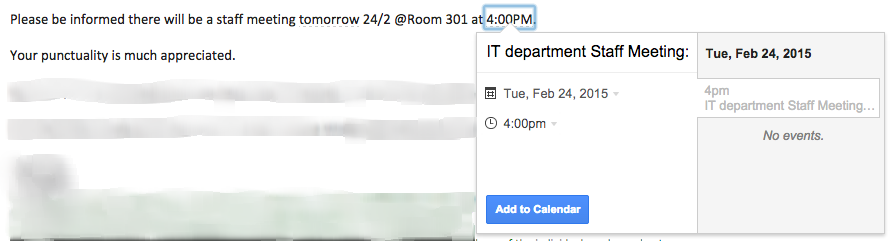
\includegraphics[width=\textwidth]{IE-event}
\end{figure}

NLP applications are often easier to design and implement with a specific use case scenario in mind

\end{frame}


\begin{frame}
\frametitle{Named Entity Recognition (NER)}

\begin{itemize}
\item Identification of proper nouns in the text
\item And classify them into catogeries of interest
\pause
\item (Typically Person, Location, Organisation, Date, Currency\ldots)
\pause
\item `\textbf{John}$_\text{PER}$ stays in \textbf{London}$_\text{LOC}$. He works there for \textbf{Polar Bear Design}$_\text{ORG}$.'
\end{itemize}

\end{frame}


\begin{frame}
\frametitle{Co-reference Resolution}

\begin{itemize}[<+->]
\item Tracking references to NEs
\item 
\tikz[baseline,remember picture]\node[anchor=base,inner sep=0pt] (john) {John}; 
stays in \tikz[baseline,remember picture]\node[anchor=base,inner sep=0pt] (london) {London};. 
\tikz[baseline,remember picture]\node[anchor=base,inner sep=0pt] (he) {He}; 
works \tikz[baseline,remember picture]\node[anchor=base,inner sep=0pt] (there) {there}; 
for Polar Bear Design. 
\tikz[overlay,remember picture]\path(he.south) edge[bend left,->,draw, >=latex'] (john.south) (there.north) edge[bend right,->,draw, >=latex'] (london.north);
\end{itemize}

\end{frame}


\begin{frame}
\frametitle{Question Answering (QA)}
\framesubtitle{e.g.~Siri}

\begin{itemize}[<+->]
\item Need to compile, index, extract a knowledge base of facts (re IE)
\item Need to analyse and interpret question to identify elements
\item Need to search knowledge base
\item May need to make inferences
\item Need to present answers in a sensible manner
\end{itemize}

\begin{columns}[T]
\begin{column}{.35\linewidth}
\begin{description}[Q:]
\item[Q:] `Where is Polar Bear Design located?'
\item[A:] London
\end{description}
\end{column}

\pause

\begin{column}{.64\linewidth}
\begin{exampleblock}{Knowledge Base}
	$\text{John}_\text{PER} \xrightarrow{\text{live-in}} \text{London}_\text{LOC}$\\
	$\text{John}_\text{PER} \xrightarrow{\text{employee-of}} \text{Polar Bear Design}_\text{ORG}$\\
	\alert{$\text{Polar Bear Design}_\text{ORG} \xrightarrow{\text{based-in}} \text{London}_\text{LOC}$}
\end{exampleblock}
\end{column}
\end{columns}

\end{frame}


\begin{frame}[allowframebreaks]
\frametitle{Plagiarism and Paraphrase Detection}
    
\begin{itemize}[<+->]
\item TurnItIn currently just detects plagiarism based on string matching
\item What about paraphrasing? Also a form of plagiarism
\item Check if several news reports are about the same event/issue
\item \parencite{li2006sentence,pera2011simpad}
\end{itemize}
\end{frame}


\begin{frame}
\frametitle{Checking the Semantic Similarity}

\url{http://swoogle.umbc.edu/StsService/GetStsSim}

\begin{itemize}
\item Inputs:
	\begin{itemize}
		\item `Many \textbf<2->{dairy} farmers today use \textbf<2->{machines} for \textbf<2->{operations} from milking to \textbf<2->{culturing} cheese.'
		\item `Today many \textbf<2->{cow} farmers perform different \textbf<2->{tasks} from milking to making \textbf<2->{cheese} using \textbf<2->{automated devices}.' 
	\end{itemize}
\item<3-> Word order, word substitutions
\item<4-> $ > 70\%$ similarity!
\end{itemize}

\end{frame}


\begin{frame}
\frametitle{Sentiment Analysis \& Opinion Mining}

\begin{itemize}
\item<1> Extract human judgement, evaluation, emotion, polarity from an utterance.
\item<1> Blogs, forum posts, tweets, speeches\ldots
\item<2> Sentimen Classfication: \url{http://text-processing.com/demo/sentiment/}
	\begin{itemize}
	\item `This movie is overrated -- all special effects, no heart.' 
		\begin{description}
			\item[Polarity] pos: 0.4; neg: 0.6 (more negative than positive)
			\item[Subjectivity] neutral: 0.2; polar: 0.8 (more subjective than objective) 
		\end{description}
	\item Negation: `It's not bad.' ???
	\end{itemize}
\item<3> More targeted:
	\begin{itemize}
	\item `The price is rather high, but the material is quite sturdy.'
	\item \texttt{[price]} -ve; \texttt{[material]} +ve
	\end{itemize}
\end{itemize}

\end{frame}

\begin{frame}
\frametitle{US 2012 Presidential Election Campaign}
    
\begin{itemize}
\item \citetitle{wang2012system} \parencite{wang2012system}
\item Twitter index tracks sentiment on Obama, Romney \href{http://usatoday30.usatoday.com/news/politics/story/2012-08-01/twitter-political-index/56649678/1}{\beamergotobutton{Link}}
\item How Social Media Sentiment Impacts the Presidential Campaigns \href{http://contently.com/strategist/2012/10/24/social-media-sentiment-becomes-factor-in-presidential-campaigns/}{\beamergotobutton{Link}}
\item Tracking sentiments of a speech \href{http://sentiment.dev.ber.to/}{\beamergotobutton{Link}}
\end{itemize}

\end{frame}


\begin{frame}
\frametitle{Speech Recognition and Synthesis}

\begin{itemize}[<+->]
\item Speech recognition: speech-to-text (STT)
	\begin{itemize}
	\item Accents, non-native speakers, pauses, filler noises\ldots
	\end{itemize}
\item Speech synthesis: text-to-speech (TTS)
	\begin{itemize}
	\item Easier? (bank teller systems etc)
	\item How to simulate \alert{natural sounding} speech?
	\end{itemize}
\end{itemize}

\end{frame}

\begin{frame}
\frametitle{Speech Recognition $\neq$ Voice Recognition}
\begin{itemize}[<+->]
\item Speech recognition
	\begin{itemize}
	\item Given a speech sample, what was said? `Dubai' or `Good bye'?
	\item Involves language modelling (statistical model of valid sentences)
	\end{itemize}
\item Voice recognition
	\begin{itemize}
	\item Given a speech sample, determine the identity of speaker
	\item Involves signal processing, voice signatures
	\end{itemize}
\end{itemize}
\end{frame}

\begin{frame}
\frametitle{Two Approaches} 
\begin{itemize}
\item Signal processing $\longrightarrow$ identify phonemes (sound units)
\item Language modelling $\longrightarrow$ likelihood of utterance
	\begin{itemize}
	\item `It's fun to recognize speech' or
	\item `It's fun to wreck a nice beach'
	\end{itemize}
\end{itemize}
\end{frame}
%!TEX root = Intro-NLP-seminar.tex
\section{NLP Processing Layers}

\begin{frame}
\frametitle{Linguistic Layers in NLP}

\centering

\begin{tabular}{c @{ $\Longleftrightarrow$ } c}
Morphology & word formation\\
Syntax & sentence structure, grammar\\
Semantics & meaning\\
Pragmatics & discourse, context\\[1em]
Speech & phonemes (speech units)
\end{tabular}

\end{frame}

\plain{Examples here are for English -- other languages may need different approaches}


\subsection{Morphology}

\begin{frame}
\frametitle{Morphology}
\begin{itemize}[<+->]
	\item How words are formed
		\begin{description}[Derivation:]
			\item[Inflection:] plant $\longrightarrow$ plants, planted, planting \ldots 
			\item[Derivation:] plant $\longrightarrow$ plantation, implant \ldots
		\end{description}
	\item For Malay:
		\begin{description}[Derivation:]
		\item[Inflection:] sakit $\longrightarrow$ sakitnya; pergi $\longrightarrow$ pergilah
		\item[Derivation:] sakit $\longrightarrow$ pesakit, penyakit, sakitan\ldots
		\end{description}
	\item Morphology processing: related to words
\end{itemize}
\end{frame}


\begin{frame}
\frametitle{Tokenising}

\begin{itemize}[<+->]
	\item Split input text into processable units
	\item Just by space characters\ldots?
		\begin{itemize}
			\item 
			\tikz[baseline, start chain=going right, node distance=0.5em, every node/.style={on chain, draw, text height=1.25ex, text depth=.25ex}]
			\path node{Passers-by} node{didn't} node{go} node[draw=none]{\ldots};
		\end{itemize}
	\item Just by punctuation/word boundaries\ldots?
		\begin{itemize}
			\item \tikz[baseline, start chain=going right, node distance=0.5em, every node/.style={on chain, draw, text height=1.25ex, text depth=.25ex}]
			\path node{Passers} node{-} node{by} node{didn} node{'} node{t} node{go} node[draw=none]{\ldots};
		\end{itemize}
	\item \alert{Tokenizers need to consider natural language!}
		\begin{itemize}
			\item \tikz[baseline, start chain=going right, node distance=0.5em, every node/.style={on chain, draw, text height=1.25ex, text depth=.25ex}]
			\path node{Passers-by} node{did} node{n't} node{go} node[draw=none]{\ldots};

		\end{itemize}
\end{itemize}

\end{frame}


\begin{frame}
\frametitle{Sentence Splitting}
\begin{itemize}
	\item How to identify sentence boundaries?
	\item ``That's wonderful,' he said. `Have your people call mine. Try to arrange something by 10 a.m. tomorrow.''
\end{itemize}
\end{frame}


\begin{frame}[allowframebreaks]
\frametitle{Stemming}
    
\begin{itemize}
\item \textbf{Stem:} reduced form (word stem, base or root form) or a word
\item Need not be identical to the morphological root of the word!
\item As long as related words map to the same stem
\item Usually implemented by stripping prefix/suffix

\framebreak

\item Example stemming:
	\begin{itemize}
	\item carresses $\rightarrow$ carress
	\item ponies $\rightarrow$ poni
	\item caress $\rightarrow$ caress
	\item cats $\rightarrow$ cat
	\item producer $\rightarrow$ produc
	\item produced $\rightarrow$ produc
	\item producing $\rightarrow$ produc
	\end{itemize}

\item Can have phases/sequences of rules \parencite{porter:1980,paice:1994}
\end{itemize}

\end{frame}

\begin{frame}
\frametitle{Why Stemming?}
    
\begin{itemize}[<+->]
\item Information Retrieval -- search for documents based on keywords
\item Stem all words in documents and store as index
\item Input keyword: producer $\rightarrow$ `produc'
\item Search documents whose indices contain `produc'
\item Results will include documents containing `produce', `produced', `producer' \ldots
\end{itemize}

\end{frame}


\begin{frame}[allowframebreaks]
\frametitle{Lemmatising}

\begin{itemize}
\item \textbf{Lemma:} base form of a word or term that is used as the \emph{formal dictionary entry} for the term.
\item Lemmatising can be seen as a special form of stemming
	\begin{itemize}
	\item Stemming: outputs do not need to be real words
	\item Lemmatising: outputs are genuine words used as headwords in dictionaries
	\end{itemize}
\end{itemize}

\ex
\begingl
\gla \textsmaller{Input:} banks raised rates to fight inflation//
\glb \textsmaller{Lemmas:} bank raise rates to fight inflation//
\endgl
\xe
\end{frame}


\begin{frame}
\frametitle{Stemming vs Lemmatising}
    
\begin{itemize}
\item Stemming is much faster than lemmatising
\item But lemmatising is essential for many NLP tasks
\end{itemize}

\end{frame}

\begin{frame}
\frametitle{Would lemmatising be required for these languages?}

\begin{itemize}
\item Malay
\item Chinese
\end{itemize}

\end{frame}


\begin{frame}
\frametitle{Segmentation}
\begin{itemize}[<+->]
\item Languages without word boundaries, e.g.~Chinese, Thai, Japanese, German\ldots
\item Essential for proper understanding!
\item Chinese example: {\xiheifont 有职称的和尚未有职称的}

\ex
\xiheifont
\begingl
\gla 有 职称 的 和 尚未 有 职称 的//
\glb with position ones and {not yet} with position ones//
\endgl
\xe

\ex
\xiheifont
\begingl
\gla 有 职称 的 \alert{和尚} 未有 职称 的//
\glb with position ones \alert{monks} without position ones//
\endgl
\xe

\end{itemize}

\end{frame}


\begin{frame}
\frametitle{Technological readiness}
    
\begin{itemize}
\item For English: libraries exists to perform these tasks
\item For other languages: depends -- some are still under research and development
\end{itemize}

\end{frame}

\subsection{Syntax}

\begin{frame}
\frametitle{Syntax}
\begin{itemize}
\item How words \emph{form phrases and sentences}
\item Grammatical rules and structures!
\item Syntactic processing: extract structure of phrase/sentences
\end{itemize}
\end{frame}


\begin{frame}[allowframebreaks]
\frametitle{Part-of-Speech (POS)}

\begin{itemize}[<+->]
\item A category assigned to a word based on its grammatical and semantic properties.
\item Example: noun, verb, adjective, adverb, determiner, preposition\ldots
\item Different languages may have different sets of POS e.g.~classifier (penjodoh bilangan)
%\item Open-class words (content words): nouns, verbs, adjectives, adverbs
%\item Closed-class words (function words): determiners, pronouns, conjunctions, infinitives\ldots
\end{itemize}
\end{frame}

\begin{frame}
\frametitle{POS Tagset}
\begin{itemize}
\item English: Penn Treebank (PTB) tagset is widely adopted \parencite{marcus1993building}
\item \url{https://www.ling.upenn.edu/courses/Fall_2003/ling001/penn_treebank_pos.html}
\end{itemize}
 
\begin{center}
\begin{tabular}{ll}
\toprule
Tag & Description\\
\midrule
NN & Noun, singular or mass\\
NNS & Noun, plural\\
VB & Verb, base form\\
VBD & Verb, past tense\\
VBG & Verb, gerund or present participle\\
\ldots & \ldots\\
\bottomrule
\end{tabular}
\end{center}

\end{frame}


\begin{frame}
\frametitle{POS-tagging}
    
\begin{itemize}
\item Given an utterance, assign the most likely POS tag to each word token
\item Current libraries quite stable now (for English): $\sim 96\%$ accuracy
\end{itemize}

\ex\deftagex{basic}
\begingl
\gla \textsmaller{Input:} banks raised rates to fight inflation//
\glb \textsmaller{POS-tags:} NNS VBD NNS TO VB NN//
\endgl
\xe 

\end{frame}


\begin{frame}
\frametitle{Phrase and Sentence Structure}
    
\begin{itemize}[<+->]
\item Sentences/clauses are made up of \emph{phrases} following grammar (syntax) rules
\item Some examples:
\begin{itemize}
\item Noun phrase (NP): `a bright star', `cats', `stars and moons'
\item Verb phrase (VP): `ran', `pick the ball up'
\item Clause/sentence (S): NP VP `a bright star pick the ball up'
\end{itemize}
\item (A syntactically correct sentence doesn't guarantee it makes sense!)
\end{itemize}

\end{frame}


\begin{frame}[fragile]
\frametitle{Shallow parsing (chunking)}

\begin{itemize}

\item Identify the noun phrases, verb phrases etc but do not go into the internal structure

\begin{multicols}{2}
\begin{tikzpicture}[transform shape, scale=.8]
\Tree [.S [.NP \edge[roof]; banks ] 
	[.VP \edge[roof]; {raised rates} ] 
	[.VP \edge[roof]; {to fight inflation} ]
]
\end{tikzpicture}

\pause
\begin{tikzpicture}[transform shape, scale=.8]
\Tree [.S [.NP \edge[roof]; {A bright star} ] 
	[.VP \edge[roof]; {pick the ball up} ] 
]
\end{tikzpicture}

\end{multicols}

\end{itemize}
\end{frame}

\begin{frame}[fragile]
\frametitle{Parsing (deep parsing)}

\begin{itemize}
\item Fully building the clauses and relations in a sentence
\item Syntactic parse tree:
\begin{multicols}{2}
`Banks raised rates to fight inflation'

{\small
\begin{verbatim}
(S
  (NP (NNS banks))
  (VP (VBD raised)
    (NP (NNS rates))
    (S
      (VP (TO to)
        (VP (VB fight)
          (NP (NN inflation)))))))
\end{verbatim}
}

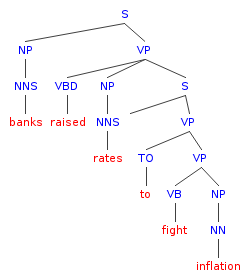
\includegraphics[width=\linewidth]{syntax-tree}

\end{multicols}
\end{itemize}
\end{frame}


\begin{frame}[fragile]
\frametitle{Dependency parsing}

\begin{itemize}
\item Find dependency relations in the text
\end{itemize}

\begin{multicols}{2}
`Banks raised rates to fight inflation'

{\small
\begin{verbatim}
nsubj(raised, banks)
root(ROOT, raised)
dobj(raised, rates)
aux(fight, to)
vmod(raised, fight)
dobj(fight, inflation)
\end{verbatim}
}

\begin{tikzpicture}[transform shape]
\Tree [.raised 
	banks
	rates
	[.fight to inflation ]
]
\end{tikzpicture}

\pause

\begin{itemize}
\item `banks' is subject of `raised'
\item `rates' is object of `raised'
\item \ldots
\end{itemize}

\end{multicols}

\end{frame}


\begin{frame}
\frametitle{Technological Readiness}
    
\begin{itemize}
\item Parsing is more difficult than POS-tagging
\item But largely solved for English
\item Varies for other languages (e.g.~OK for Chinese, no truly satisfactory one yet for Malay)
\end{itemize}

\end{frame}

\subsection{Semantic}

\begin{frame}
\frametitle{Semantic}

\begin{itemize}
\item The meaning conveyed by the text
\item Hard!
\item How to represent `meaning'?
\item Still an open question in articifial intelligence, cognitive science, psychology\ldots
\item Lots of on-going research
\end{itemize} 

\end{frame}


\begin{frame}
\frametitle{Word Sense}
    
\begin{itemize}
\item One of zero to many \emph{meanings or concepts} associated with a given \emph{head word/lemma}, as listed in a specific lexicon
\item Lexicon: a machine-readable, structured dictionary
\item May also include relations between word senses
	\begin{itemize}
	\item Synonyms, antonyms, is-a-type-of\ldots
	\end{itemize}
\end{itemize}

\end{frame}


\begin{frame}
\frametitle{Synonym Expansion}
    
\begin{itemize}
\item Example in information retrieval (search engine)
\item Search for `wizard' would also retrieve documents containing `sorcerer', `magician'
\end{itemize}

\end{frame}


\begin{frame}
\frametitle{Word Sense Disambiguation (WSD)}

\begin{itemize}
\item a.k.a.~Sense-tagging
\item Associating a word occurrence with its most likely sense, with repect to a specific lexicon
\item \textbf{Stop words:} Words that are ignored in NLP tasks, e.g.~function words in a sense-tagging task.
\end{itemize}
\end{frame}

\begin{frame}
\frametitle{How to identify stop words?}

\begin{itemize}
\item Open-class words (content words): nouns, verbs, adjectives, adverbs
\item Closed-class words (function words): determiners, pronouns, conjunctions, infinitives\ldots
\end{itemize}

\ldots so WSD needs POS-tagging and lemmatisation first

\end{frame}

\begin{frame}
\frametitle{WSD Example}

\begin{exampleblock}{Senses of bank.n in WordNet}
\begin{enumerate}
\item sloping land (especially the slope beside a body of water)
\item a financial institution that accepts deposits and channels the money into lending activities
\item a long ridge or pile
\item \ldots
\end{enumerate}
\end{exampleblock}

\ex\deftagex{basic}
\begingl
\gla \textsmaller{Input:} banks raised rates to fight inflation//
\glb \textsmaller{Sense-tags:} bank.n.2 raise.v.13 rates.n.1 {} fight.v.1 inflation.n.1//
\endgl
\xe     
\end{frame}


\begin{frame}
\frametitle{Concept Tagging}
    
\begin{itemize}
\item Label each sense in the input with a concept tag \\
(Example below uses WordNet--SUMO mapping)
\end{itemize}

\lingset{everyglb={\footnotesize}, everyglc={\scriptsize\scshape}}
\ex\deftagex{basic}
\begingl
\gla \textsmaller{Input:} banks raised rates to fight inflation//
\glb \textsmaller{Sense-tags:} bank.n.2 raise.v.13 rates.n.1 {} fight.v.1 inflation.n.1//
\glc \textsmaller{\upshape Concept tags:} Corporation Increasing Tax {}  ViolentContest Increasing//
\endgl
\xe 

\end{frame}


\begin{frame}
\frametitle{Information Extraction}

\begin{itemize}
\item Examples as given earlier
\item Named entity recognition
\item Coreference resolution
	\begin{itemize}[<+->]
	\item `The cat climbed onto the chair. It yawned and slept.'
	\item `It' = `the cat'? `the chair'?
	\item `cat' $\xrightarrow{\text{is-a}}$ \textsc{animal} $\xrightarrow{\text{is-a}}$ \textsc{animate object}
	\item `chair' $\xrightarrow{\text{is-a}}$ \textsc{furniture} $\xrightarrow{\text{is-a}}$ \textsc{inanimate object}
	\item \textsc{animate object} $\xrightarrow{\text{capable-of}}$ `yawn', `sleep'
	\item $\therefore$ `It' = `the cat'
	\end{itemize}
\end{itemize}

\end{frame}



\subsection{Pragmatics}

\begin{frame}
\frametitle{Pragmatics}

\begin{itemize}[<+->]
\item Processing text by inclduing context
\item Scenario, behavior, cultural, etc
	\begin{description}[<+->]
	\item[Q] `Can you pass me the salt?'
	\item[Machine] `Yes.'
	\item[Human] [picks up salt shaker and hands over]
	\end{description} 
	\begin{description}[<+->]
	\item[Teacher] `This is your assignment.'
	\item[Student] `What is assignment? Can eat one ah?'
	\item[Machine] `An assignment is your homework. It is not edible.'
	\item[Teacher] [rolls eyes and ignores comment]
	\end{description} 
\item `He opened the fridge.' (because he was hungry?)
\item \textbf{VERY HARD!!!}
\end{itemize}

\end{frame}


\begin{frame}
\frametitle{Speech}

\begin{itemize}[<+->]
\item Existing libraries: Android, eSpeak, Microsoft SAPI\ldots
\item Support for English is satisfactory for FYP purposes
\item (Not so good for other languages especially recognition)
\item Sounds mechanical!
\item Prosody: more natural-sounding, with emotions etc (R\&D!)
\end{itemize}
\end{frame}


% \begin{frame}
% \frametitle{Speech Synthesis: More Details}
% \begin{itemize}[<+->]
% \item Basic unit: \alert{phonemes}
% \item Speech synthesis common steps:
% 	\begin{itemize}
% 	\item Look up pronunciation coding in dictionary\\
% 		e.g.~SAMPA phonemes (MBROLA); Krishenbaum (eSpeak)\\
% 	\item `This is some phonetic text input'
% 	\item \lstinline|D,Is Iz sVm f@n'EtIk t'Ekst 'InpUt|
% 	\end{itemize}
% \end{itemize}

% \end{frame}
%!TEX root = Intro-NLP-seminar.tex

\section{Example Individual Projects using NLP}

\begin{frame}
\frametitle{Translator Aid for Travellers}
    
\centering
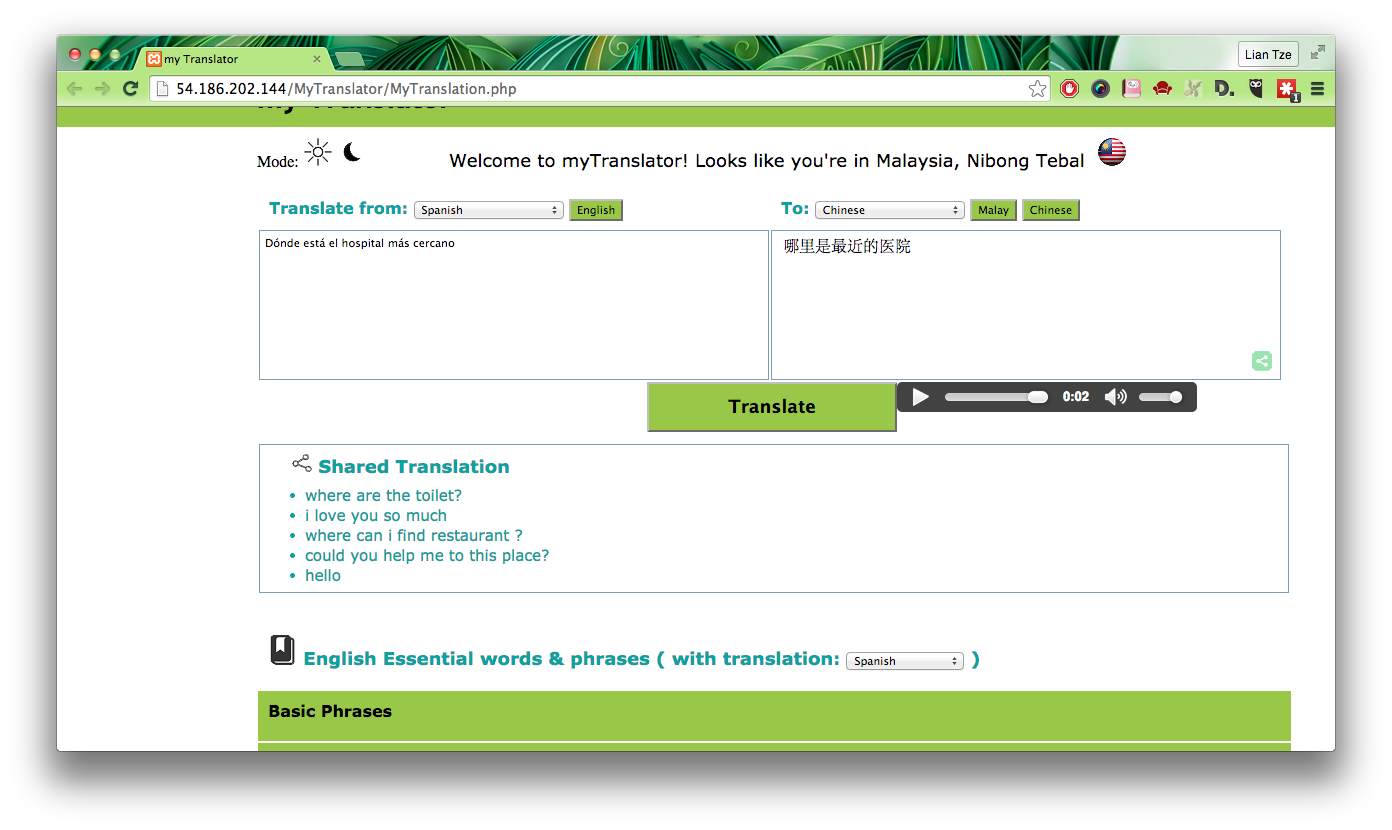
\includegraphics[width=\textwidth]{mytranslator}

\end{frame}


\begin{frame}
\frametitle{Bloom's Taxonomy Level Categorisation}
    
\centering
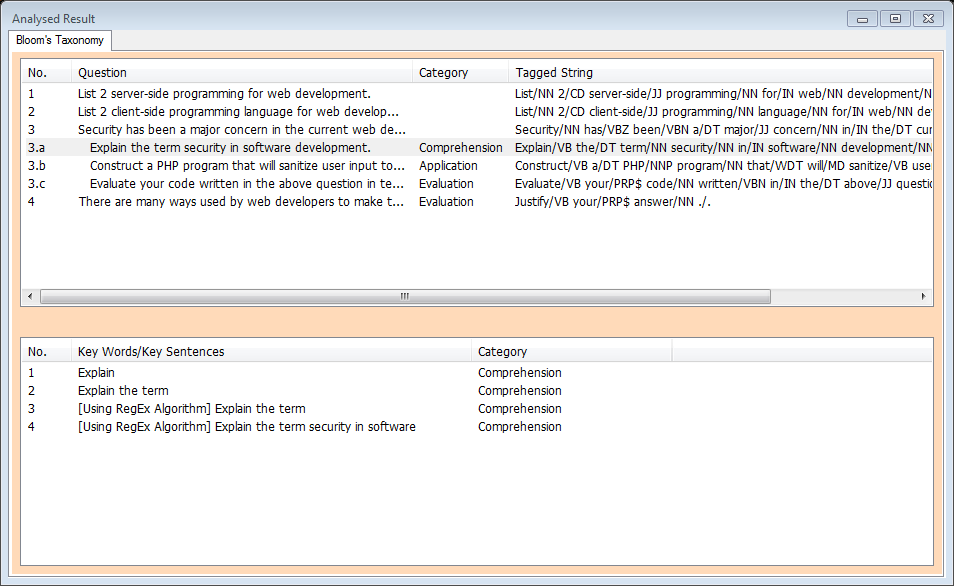
\includegraphics[width=\textwidth]{bloom-debug}

\end{frame}


\begin{frame}
\frametitle{More Examples}
    
\begin{itemize}
\item Named entity recognition including Malaysian names
\item Intelligent meaning lookup for mixed language input with spelling error detection
\item *Sentiment analysis of forum posts
\item *Information extraction to identify problem parameters
\item *Keyword extraction from paper publications
\end{itemize}
 
\end{frame}

%\begin{frame}
%\frametitle{Named Entity Recognition for Malay}
%\end{frame}


%\begin{frame}
%\frametitle{Intelligent Lookup with Mixed-language Input}
%\end{frame}
\plain{End of Session 1\\See you next week!}
%!TEX root = Intro-NLP-seminar.tex
\section{Code Samples for Common Tasks in NLP}

\begin{frame}
\frametitle{What Programming Languages Can I Use for NLP?}
    
\begin{description}
\item[Java] Apache OpenNLP, \textbf<2>{Stanford NLP}, Lucene, GATE, LingPipe\ldots
\item[Python] NLTK (with a nice textbook)
\item[.NET, PHP] \textbf<2>{Stanford NLP}, Lucene\ldots
\end{description}

%(Java and C\#.NET works quite well)

\uncover<2>{Demonstration: Java and PHP, mostly using Stanford's libraries}

\end{frame}


\subsection{Stemming}

\begin{frame}
\frametitle{Libraries for Stemming}
    
\begin{itemize}
\item Many libraries available \\\url{http://tartarus.org/martin/PorterStemmer/}
\item Or implement your own -- nice scope for Individual Project
\item \textcite{porter:1980} is most famous but there are other algorithms too
\end{itemize}

\end{frame}

\begin{frame}[fragile,allowframebreaks]
\frametitle{Stemming Demo using PorterStemmer.class.php}
    
\begin{lstlisting}[language=PHP]
<?php
    require_once('PorterStemmer.class.php');

    $stem = PorterStemmer::Stem("cats");
    echo "$stem<br/>\n";
    $stem = PorterStemmer::Stem("ponies");
    echo "$stem<br/>\n";
    $stem = PorterStemmer::Stem("produce");
    echo "$stem<br/>\n";
    $stem = PorterStemmer::Stem("producer");
    echo "$stem<br/>\n";
    $stem = PorterStemmer::Stem("producing");
    echo "$stem<br/>\n";
?>
\end{lstlisting}
\end{frame}

\begin{frame}[fragile]
\frametitle{Stemmer Output}

\begin{lstlisting}[columns=fullflexible]
cat
poni
produc
produc
produc
\end{lstlisting}

\end{frame}

\subsection{Stanford Parser}


\begin{frame}
\frametitle{Stanford Parser}

\begin{itemize}
\item \parencite{stanford:parser:2003}
\item Stanford Parser can POS-tag, lemmatize \emph{and} parse!
\item Not always the best results, but widely used \Winkey
\end{itemize}    

\end{frame}



\begin{frame}
\frametitle{Installing and Setting Up}

\begin{description}[Java]

\item[Java]
	\begin{itemize}
	\item Download the Java library from \url{http://nlp.stanford.edu/software/lex-parser.shtml}
	\item Unzip and place somewhere on system e.g.~in \directory{C:/}\\[1em]
	\end{itemize}

\item[PHP]
	\begin{itemize}
	\item Download the Java library first
	\item Download the PHP library from \url{https://github.com/agentile/PHP-Stanford-NLP}
	\item Unzip and place in \directory{C:/xampp/htdocs}\\[1em]
	\end{itemize}

\item[.NET]
	\begin{itemize}
	\item Download the Java library first
	\item Follow instructions at \url{http://sergey-tihon.github.io/Stanford.NLP.NET/}
    \item Class names, function calls etc.~exactly same as Java API
	\end{itemize}
\end{description}

\end{frame}

\begin{comment}
\begin{frame}[fragile]
\frametitle{Java Code Sample (Adapted from TaggerDemo.java)}
    
\begin{lstlisting}[language=Java,basicstyle={\ttfamily\scriptsize},gobble=4,
	morekeywords={String, MaxentTagger, List}]
    String model = "models/english-bidirectional-distsim.tagger";
        String text = "This is some text with many sentences and words. " 
                + "We use it to test our programs.";

    // Initialise the POS tagger
    MaxentTagger tagger = new MaxentTagger(model);

    // Pre-processing: sentence-splitting and tokenising
    List<List<HasWord>> sentences = MaxentTagger.tokenizeText(
        new BufferedReader(new StringReader(text)));

    // Loop through list of sentences
    for (List<HasWord> sentence : sentences) {
    	// POS-tag each sentence
        List<TaggedWord> tSentence = tagger.tagSentence(sentence);

        // Loop through each tagged word
        for (TaggedWord tw: tSentence) {
            System.out.print( tw.word() + "/" + tw.tag() + " " );
        }
        System.out.println();
    }
\end{lstlisting}

\end{frame}

\begin{frame}[fragile]
\frametitle{POS-Tagging Output}
    
\begin{lstlisting}[basicstyle=\ttfamily\footnotesize]
This/DT is/VBZ some/DT text/NN with/IN many/JJ sentences/NNS and/CC words/NNS ./. 
We/PRP use/VBP it/PRP to/TO test/VB our/PRP$ programs/NNS ./. 
\end{lstlisting}

Refer to PTB tagset\\
\url{https://www.ling.upenn.edu/courses/Fall_2003/ling001/penn_treebank_pos.html})

\end{frame}

\begin{frame}[fragile]
\frametitle{POS-Tagging Code Sample for PHP}

\begin{lstlisting}[language=PHP,basicstyle=\ttfamily\footnotesize,showtabs=true,tabsize=4]
<?php
require_once('autoload.php');

// Note that the PHP version can only tag single sentence
// (Write your own splitting function using regular expression)
$text = "This is some text with many sentences and words.";

// Copy these files from the Java version to current folder
$pos = new \StanfordNLP\POSTagger(
	'english-bidirectional-distsim.tagger','stanford-postagger.jar');

$results = $pos->tag(explode(' ', $text));

// Loop through the list of tagged words
foreach ($results as $tagged) {
	// each $tagged is an array: word and tag
	echo "$tagged[0]/$tagged[1] ";
}
echo "<br/>";
?>
\end{lstlisting}


\end{frame}
\end{comment}

%\subsection{Lemmatising}

\subsection{POS-Tagging and Lemmatising}

\begin{frame}[fragile,allowframebreaks]
\frametitle{Java Code Sample}

(\small Make sure \texttt{stanford-parser.jar} and \texttt{stanford-parser-\emph{version}-models.jar} are in the library path)


\begin{lstlisting}[language=Java,basicstyle={\ttfamily\footnotesize}, gobble=4,
    morekeywords={String, LexicalizedParser, List,DocumentPreprocessor,Tree,HasWord,Morphology,StringReader},
    emph={apply,getLeaves,value,parent,lemmaStatic}, frame=lines,
    escapechar=|]
    // Initialise the parser using the English model
    String parserModel = "edu/stanford/nlp/models/lexparser/englishPCFG.ser.gz";
    LexicalizedParser lp = LexicalizedParser.loadModel(parserModel);

    // Text to be processed
    String text = "26 interested students came to the seminar. " 
            + "They signed up quickly.";

    // DocumentPreprocessor performs sentence-splitting and tokenising
    for (List<HasWord> sentence : new DocumentPreprocessor(
        new StringReader(text))) {

        // Apply the parser on each sentence
        Tree parse = lp.apply(sentence);

        // Just need POS-tag and lemma?
        for (Tree leaf : parse.getLeaves()) {
            String surfaceForm = leaf.value();
            String pos = leaf.parent(parse).value();
            String lemma = Morphology.lemmaStatic(surfaceForm, pos, true);
            System.out.print(surfaceForm);
            System.out.print("/");
            System.out.print(lemma);
            System.out.print("/");
            System.out.print(pos);
            System.out.print(" ");
        }
        System.out.println();
    }
\end{lstlisting}

\end{frame}

\begin{frame}[fragile]
\frametitle{POS-Tagging and Lemmatising Output}
    
\begin{lstlisting}
23/23/CD interested/interested/JJ students/student/NNS came/come/VBD to/to/TO the/the/DT seminar/seminar/NN ././. 

They/they/PRP signed/sign/VBD up/up/RP quickly/quickly/RB ././. 
\end{lstlisting}

\end{frame}


\begin{frame}[fragile,allowframebreaks]
\frametitle{PHP Code Sample}

\lstset{morecomment=[s][\color{PaleVioletRed4}]{/*}{*/}}
\begin{lstlisting}[language=PHP,basicstyle={\ttfamily\small},
morekeywords={new}]
<?php
require_once('autoload.php');

// Initialise the parser. 
// Put the .jar files somewhere suitable
$parser = new \StanfordNLP\Parser('stanford-parser.jar', 
    'stanford-parser-3.5.0-models.jar');

$text = "26 interested students came to the seminar. " 
        . "They signed up quickly.";

// parse the text
$result = $parser->parseSentence($text);



/* var_dump $result and you'll see it's an array with 
 * 3 outputs: wordsAndTags, penn, typedDependencies */
var_dump($result);

// If only POS tag and lemma are required:
echo "<ul>";
foreach ($result["wordsAndTags"] as $tagged) {
    // each item is an array of the word and POS
    echo "<li>$tagged[0] ($tagged[1])";
}
echo "</ul>";
?>
\end{lstlisting}

\end{frame}


\begin{frame}[fragile]
\frametitle{It doesn't work on my Windows machine!}
    
\lstset{language=PHP,frame=single,basicstyle=\ttfamily\small,gobble=4}

\begin{itemize}
    \item Error: \texttt{Notice: Undefined offset: 1...}
    \item Solution: Modify \texttt{Parser.php}

    \begin{lstlisting}
    $output = explode("\n\n", trim($this->getOutput()));
    \end{lstlisting}

    to

    \begin{lstlisting}
    $output = explode("\r\n\r\n", trim($this->getOutput()));
    \end{lstlisting}

\end{itemize}

\end{frame}


\begin{frame}[fragile]
\frametitle{The PHP version doesn't return lemmas?}
    
Need to modify \texttt{Parser.php} by adding a line:

\begin{lstlisting}[language=PHP,gobble=8,escapechar=|,basicstyle=\ttfamily\small,frame=lines]
        $cmd = $this->getJavaPath()
            . " $options -cp \""
            . $this->getJar()
            . $osSeparator
            . $this->getModelsJar()
            . '" edu.stanford.nlp.parser.lexparser.LexicalizedParser -encoding UTF-8 -outputFormat "'
            . $this->getOutputFormat()
            . "\" "
            |\textbf{\color{PaleVioletRed4}. '-outputFormatOptions "stem" '}|
            . $parser
            . " "
            . $tmpfname;
\end{lstlisting}

\end{frame}

\begin{frame}
\frametitle{POS-Tagging and Lemmatising Output}
    
\begin{itemize}
\item 26 (CD)
\item interested (JJ)
\item student (NNS)
\item come (VBD)
\item to (TO)
\item the (DT)
\item seminar (NN)
\item . (.)
\end{itemize}

\end{frame}

\begin{frame}
\frametitle{PHP version returns only the 1st sentence?}
    
\begin{itemize}
\item The PHP version only captures the output for 1st sentence
\item Possible to modify \texttt{Parser.php} to return output for all sentences
\item (Try yourself or see me if needed)
\end{itemize}

\end{frame}

\subsection{Parsing}

\begin{frame}
\frametitle{Which parsing structure to use?}

\begin{itemize}
\item If you need to use the tree structure of a text -- I'd recommend the \alert{dependency} structure
\item Shorter tree; shows parent-child between word/lemmas in text
\end{itemize}
\end{frame} 


\begin{frame}[fragile,allowframebreaks]
\frametitle{Java Code Sample}
    
\begin{lstlisting}[language=Java,basicstyle=\ttfamily\footnotesize,gobble=8,
    emph={parse,lp,typedDependenciesCCprocessed,lemmaStatic,dep,gov,reln,index,tag,value},
    morekeywords={TreebankLanguagePack,GrammaticalStructureFactory,GrammaticalStructure,
        List,TypedDependency,IndexedWord,String,Morphology},
        escapechar=|]
        // Continue from earlier Java code 
        // Use the parsed tree to get the typed dependencies
        TreebankLanguagePack tlp = lp.treebankLanguagePack();
        GrammaticalStructureFactory gsf = tlp.grammaticalStructureFactory();
        GrammaticalStructure gs = gsf.newGrammaticalStructure(parse);
        List<TypedDependency> tdl = gs.typedDependenciesCCprocessed();

        // Let's just print out each of the parent-child relationship first
        for (TypedDependency td : tdl) {
            // parent = "governer"
            IndexedWord parent = td.gov();
            String parentWord = parent.value();
            String parentPOS = parent.tag();
            String parentLemma = Morphology.lemmaStatic(
                parentWord, parentPOS, true);
            
            |\framebreak|
            // child = "dependent"
            IndexedWord child = td.dep();
            String childWord = child.value();
            String childPOS = child.tag();
            String childLemma = Morphology.lemmaStatic(
                childWord, childPOS, true);
            
            
            System.out.println(
                "[" + parent.index() + "]" + parentLemma + "/" + parentPOS 
                + " <--" + td.reln().getShortName() + "-- "
                + "[" + child.index() + "]" + childLemma + "/" + childPOS);
        }
        System.out.println();
\end{lstlisting}

\end{frame}


\begin{frame}[fragile]
\frametitle{Dependencies as a List}
    
\begin{lstlisting}[basicstyle=\ttfamily\small]
[3]student/NNS <--num-- [1]23/CD
[3]student/NNS <--amod-- [2]interested/JJ
[4]come/VBD <--nsubj-- [3]student/NNS
[0]root/null <--root-- [4]come/VBD
[7]seminar/NN <--det-- [6]the/DT
[4]come/VBD <--prep-- [7]seminar/NN

[2]sign/VBD <--nsubj-- [1]they/PRP
[0]root/null <--root-- [2]sign/VBD
[2]sign/VBD <--prt-- [3]up/RP
[2]sign/VBD <--advmod-- [4]quickly/RB
\end{lstlisting}

\end{frame}


\begin{frame}[fragile]
\frametitle{Recursively Navigating the Dependency Tree}
    
\begin{lstlisting}[language=Java,basicstyle=\ttfamily\footnotesize]
// recursively go through parent-children links, starting from root
int curParent = 0;
processChildren(curParent, tdl);
System.out.println();

private static void processChildren(int parentID, List<TypedDependency> tdl) {
    for (TypedDependency td: tdl) {
        if (td.gov().index() == parentID) {
            IndexedWord childNode = td.dep();
            // do the processing with childNode's values, example:
            // Remember to lemmatise if necessary!!
            System.out.println("Child of node " + parentID + ": ["  
                + childNode.index() + "] " +  childNode.word() + "/" + childNode.tag());
            // then process childNode's children...
            processChildren(childNode.index(), tdl);
        }
    }   
}
\end{lstlisting}

\end{frame}


\begin{frame}[fragile]
\frametitle{Navigating Parent-Child Output}
    
\begin{lstlisting}
Child of node 0: [4] came/VBD
Child of node 4: [3] students/NNS
Child of node 3: [1] 23/CD
Child of node 3: [2] interested/JJ
Child of node 4: [7] seminar/NN
Child of node 7: [6] the/DT

Child of node 0: [2] signed/VBD
Child of node 2: [1] They/PRP
Child of node 2: [3] up/RP
Child of node 2: [4] quickly/RB
\end{lstlisting} 

\end{frame}


\begin{frame}[fragile,allowframebreaks]
\frametitle{PHP Code Sample}
    
\begin{lstlisting}[language=PHP,basicstyle=\ttfamily\footnotesize,
emph={typedDependencies, processChildren}, escapechar={|},
morekeywords={function}]
$curParent = 0;
echo "<ul>";
processChildren($curParent, $result["typedDependencies"]);
echo "</ul>";

function processChildren($curParent, $tdl) {
    foreach ($tdl as $td) {
        $parent = explode("/", $td[0]["feature"]);
        $parentLemma = $parent[0];
        $parentPOS = $parent[1];
        $parentIndex = $td[0]["index"];

        $child = explode("/", $td[1]["feature"]);
        $childLemma = $child[0];
        $childPOS = $child[1];
        $childIndex = $td[1]["index"];
        $reln = $td["type"];

        if ($parentIndex == $curParentID) {
            // do the processing with childNode's values, example:
            echo "<li>Child of node $curParentID: [$childIndex] " 
                . "$childLemma/$childPOS</li>\n";
            // then process childNode's children...
            processChildren($childIndex, $tdl);
        }
    }
}
\end{lstlisting}

\end{frame}


\begin{frame}[fragile]
\frametitle{By default, no POS in typedDependencies?!}
    
Need to modify \texttt{Parser.php} by adding another option:

\begin{lstlisting}[language=PHP,gobble=8,escapechar=|,basicstyle=\ttfamily\small,frame=lines]
        $cmd = $this->getJavaPath()
            . " $options -cp \""
            . $this->getJar()
            . $osSeparator
            . $this->getModelsJar()
            . '" edu.stanford.nlp.parser.lexparser.LexicalizedParser -encoding UTF-8 -outputFormat "'
            . $this->getOutputFormat()
            . "\" "
            |\textbf{\color{PaleVioletRed4}. '-outputFormatOptions "stem,\textcolor{mLightBrown}{includeTags}" '}|
            . $parser
            . " "
            . $tmpfname;
\end{lstlisting}
\end{frame}


\begin{frame}
\frametitle{Output}
    
\begin{itemize}
\item    Child of node 0: [4] come/VBD
\item    Child of node 4: [3] student/NNS
\item    Child of node 3: [1] 26/CD
\item    Child of node 3: [2] interested/JJ
\item    Child of node 4: [7] seminar/NN
\item    Child of node 7: [6] the/DT
\end{itemize}

\end{frame}

\subsection{Speech Synthesis and Recognition}

\begin{frame}
\frametitle{Speech Synthesis and Recognition}
    
\begin{itemize}
\item Microsoft Speech Platform
    \begin{itemize}
        \item English, Japanese, Chinese, French, Spanish\ldots
    \end{itemize}
\item Android -- Google Speech API
    \begin{itemize}
        \item English, Spanish, Japanese, Indonesian, French, Italian, Korean, Hindi\ldots
    \end{itemize}
\item Read the comprehensive API documentations!
\end{itemize}

\end{frame}


\begin{frame}
\frametitle{A Word on Language Codes}
    
\begin{itemize}
    \item ISO-639 Standard
    \item 2-letter and 3-letter codes

\bigskip
\begin{center}
\begin{tabular}{l >{\ttfamily}c >{\ttfamily}c}
\toprule
Language & 2-letter & 3-letter\\
\midrule
English & en & eng\\
Malay & ms & msa, zsm \textsf{(Standard Malay)}\\
Indonesian & id & ind\\
Chinese & zh & zho \\
Cantonese (Yue) & & yue\\
Hokkien (Min Nan) & & nan\\
French & fr & fra\\
\ldots & \ldots & \ldots\\
\bottomrule
\end{tabular}
\end{center}
\bigskip
\end{itemize}
\end{frame}

\begin{frame}
\frametitle{Can also specify Locales}
    
\begin{itemize}
    \item Can add country code to specify locale

\begin{center}
\begin{tabular}{>{\ttfamily}c l}
\toprule
Language code & Language \\
\midrule
en-US & American English\\
en-UK & British English\\
en-AU & Australian English\\
zh-CN & Mainland China Chinese\\
zh-TW & Taiwanese Chinese\\
zh-HK & Hong Kong Chinese\\
\ldots & \ldots\\
\bottomrule
\end{tabular}
\end{center}

\item (Sometimes underscore instead of dash; sometimes given as separate arguments\ldots)

\end{itemize}
\end{frame}

\subsection{Many Others!}

\begin{frame}
\frametitle{Other examples not shown here}

\begin{itemize}
\item Stanford NER (Java, PHP, .NET)
\item If you know Python, do look up NLTK \parencite{nltk:book}
\item GATE: Available as GUI workbench and as embedded API
\item LingPipe: Some interesting libraries for working with corpora
\item \ldots Many, many more!
\end{itemize}
    


\end{frame}
%!TEX root = Intro-NLP-seminar.tex
\section{WordNets: lexical semantic networks}

\newcommand{\mysynset}[1]{\text{(#1)}}
\newcommand{\myrel}[1]{\text{\emph{\color{purple}#1}}}
\newcommand{\myword}[1]{\text{`#1'}}
\newcommand{\myconcept}[1]{\text{\scshape #1}}
\newcommand{\myinst}[1]{\text{\scshape\color{green!30!black} #1}}

\begin{frame}
\frametitle{WordNet: An Electronic Lexical Database}

\begin{itemize}
\item \parencite{miller:wordnet:1995}
\item Developed by Princeton University Cognitive Science Laboratory for (American) English
\item Lexical entries organised by \emph{meaning} (semantic content)
\item Wordnets for many other languages have been developed
%\item For humans: new ways of navigating a dictionary/lexicon to learn about words
%\item For computers: resource for performing (some level of) semantic analysis on natural language text
\end{itemize}
\end{frame}

\subsection{Synsets}
\begin{frame}
\frametitle{Synsets = ``synonym set''}
\begin{itemize}
\item Basic unit; represents a word meaning by \alert{synonyms}, \alert{gloss} and \alert{relations to other synsets}
\item Different senses of a word (collocation, phrasal verb, etc.) are placed in different synsets according to parts-of-speech
\item Each synset contains senses of different words that are considered synonymous
%\item For each synset:
%  \begin{itemize}
%    \item gloss
%    \item semantic field
%    \item example usage(s)
%    \item sentence frame (verbs only)
%  \end{itemize}
\end{itemize}
\end{frame}

\begin{frame}[fragile]
\frametitle{First 3 senses for noun ``court''}

\begin{itemize}
	\item 3 synsets, one for each sense (meaning)
	\item Each synset contain member lemmas with same meaning, same POS
	\item Each synset has a definition text; may have example sentence
\end{itemize}

\bigskip

\lstset{keywordstyle=\color{red},keywords={court}}
\begin{lstlisting}
<noun.group> court, tribunal, judicature - (an assembly (including one or more judges) to conduct judicial business)

<noun.group> court, royal_court - (the sovereign and his advisers who are the governing power of a state)

<noun.artifact> court - (a specially marked horizontal area within which a game is played; "players had to reserve a court in advance")
\end{lstlisting}

\end{frame}


\begin{frame}
\frametitle{Synset Organisation}
    
\begin{itemize}
\item 4 synset categories

\bigskip

\begin{center}
\begin{tabular}{l >{\ttfamily}c c}
\toprule
Category & POS code & numerical prefix\\
\midrule
noun & n & 1 \\
verb & v & 2 \\
adjective & a, s & 3 \\
adverb & r & 4 \\
\bottomrule
\end{tabular}
\end{center}

\bigskip

\item Primary key: 9-digit synset ID \alert{or} POS code + 8-digit synset ID
\item WN3.0 synset (court, tribunal, judicature) can be identified by \alert{108329453} or \alert{n-08329453} or \alert{08329453-n} in different systems
\end{itemize}
\end{frame}

\begin{frame}
\frametitle{Mapping Stanford Parser POS codes to WN POS code}

\begin{algorithmic}
\STATE \COMMENT{Ignore all other POS when looking up WN}
\IF{\texttt{\$stanfordPOS} starts with `N'}
	\STATE \texttt{\$wnPOS} $\leftarrow$ `n'
	\STATE \texttt{\$wnPOSnum} $\leftarrow$ 1

\ELSIF{\texttt{\$stanfordPOS} starts with `V'}
	\STATE \texttt{\$wnPOS} $\leftarrow$ `v'
	\STATE \texttt{\$wnPOSnum} $\leftarrow$ 2

\ELSIF{\texttt{\$stanfordPOS} starts with `J'}
	\STATE \texttt{\$wnPOS} $\leftarrow$ \{`a', `s'\}
	\STATE \texttt{\$wnPOSnum} $\leftarrow$ 3

\ELSIF{\texttt{\$stanfordPOS} starts with `R'}
	\STATE \texttt{\$wnPOS} $\leftarrow$ `r'
	\STATE \texttt{\$wnPOSnum} $\leftarrow$ 4
\ENDIF 
\end{algorithmic}


\end{frame}


\subsection{Relations}
\begin{frame}
\frametitle{Noun Synset Relations}
%\framesubtitle{Nouns}
%WordNet specifies relations between synsets and (compound) words

%\begin{exampleblock}{Noun Synset Relations}
\mode<presentation>{\small}
\begin{description}
\item[hypernymy] \mysynset{court, royal court} \myrel{is-a-kind-of} \mysynset{government, authorities, regime}
\item[holonymy] \mysynset{finger} \myrel{is-part-of} \mysynset{hand, manus, mitt, paw} \\
                \mysynset{flour} \myrel{is-substance-of} \mysynset{bread}, \mysynset{dough}, \mysynset{pastry} \\
                \mysynset{jury} \myrel{is-member-of} \mysynset{court, tribunal, judicature}
\item[instance] \mysynset{Mozart, Wolfgang Amadeus Mozart} \myrel{is-instance-of} \mysynset{composer}
\end{description}
(\ldots{}and their respective inverse relations)
%\end{exampleblock}
\end{frame}

\begin{frame}
\frametitle{Verb Synset Relations}
%\framesubtitle{Verbs}
%WordNet specifies relations between synsets and (compound) words

%\begin{exampleblock}{Verb Synset Relations}
\mode<presentation>{\small}
\begin{description}
\item[hypernymy] \mysynset{stroll, saunter} \myrel{is-one-way-to} \mysynset{walk}
\item[troponymy] \mysynset{fear} \myrel{has-specific-way} \mysynset{panic}
\item[cause] \mysynset{teach} \myrel{causes} \mysynset{learn, larn, acquire}
\item[entailment] \mysynset{buy, purchase} \myrel{entails} \mysynset{pay}, \mysynset{choose, take, select, pick out}
\item[verb frames] \mysynset{attack, assail}: \\\texttt{Somebody --s something}\\\texttt{Somebody --s somebody}\\(very simple, without any extra info)
\end{description}
%\end{exampleblock}
\end{frame}

\begin{frame}
\frametitle{Lexical Relations}
\mode<presentation>{\small}
\begin{description}
\item[antonymy] \myword{ugliness} \myrel{$\times$} \myword{beauty}, 
                \myword{pull} \myrel{$\times$} \myword{push},\\
                \myword{difficult} \myrel{$\times$} \myword{easy}, 
                \myword{quickly} \myrel{$\times$} \myword{slowly}
\item[attribute] \myword{strength} \myrel{has-attributes}: \myword{delicate}, \myword{rugged}, \myword{weak}, \myword{strong}
\item[derivation] \myword{maintain} \myrel{is-derivationally-related-to} \myword{maintainable}, \myword{maintenance}, \myword{maintainer}
\item[domain] \myword{medicine} \myrel{topic-has-terms}: \myword{acute}, \myword{fulgurating}, \myword{gauze}, \ldots\\
              \myword{France} \myrel{region-has-terms}: \myword{Battle of Valmy}, \myword{Bastille}, \myword{jeu d'esprit}, \ldots\\
              \myword{colloquialism} \myrel{usage-has-terms}: \myword{lousy}, \myword{humongous}, \myword{gobsmacked}, \ldots
\item[pertainym] \myword{biannual} \myrel{pertains-to} \myword{year}, 
                 \myword{ancestral} \myrel{pertains-to} \myword{ancestor},
                 \myword{Liverpudlian} \myrel{pertains-to} \myword{Liverpool}
\item[participle] \myrel{a} \myword{handheld} \myrel{something-participates-in} \myword{hold}
\end{description}
\end{frame}

\subsection{Getting the Data}

\begin{frame}
\frametitle{Princeton WordNet Data}
    
\begin{itemize}[<+->]
\item Browse/explore online: \url{http://wordnet.princeton.edu/}
\item Searching WordNet: APIs for many programming languages available
\item \ldots But I recommend downloading WordNet as MySQL data
\item Then use whatever programming language you like to query
\end{itemize}

\end{frame}


\begin{frame}[fragile]
\frametitle{WordNet SQL}
    
\begin{itemize}
\item \url{http://wnsql.sourceforge.net/}
\item \menu{Download > wnsql > mysql > 3.0 > mysql-3.0.0-30-wn-30.zip} Unzip. 
\item Create a MySQL database, e.g.~ \texttt{wordnet30}
\item Start a Windows command prompt.\\\menu{Windows Start > Run} type \menu{cmd} \return

\begin{lstlisting}[backgroundcolor=\color{black},basicstyle=\ttfamily\color{green}, 
escapechar=|, framexleftmargin=1em, xleftmargin=1em]
> cd <folder containing unzipped contents> |\return|
> restore.bat |\return|
\end{lstlisting}

\item You'll be prompted for the database name, username and password. Wait while the data is copied into tables.

\item (May need to add \path{C:\xampp\mysql\bin} to system path)
\end{itemize}

\end{frame}



\begin{frame}[fragile]
\frametitle{Some Tables in WN-MySQL}
    
\begin{tikzpicture}[every node/.style={rectangle split, rectangle split parts=2, draw},
every text node part/.style={align=center}] 
\node (words) [text width=4em] 
{words \nodepart{two}{\textbf{wordid}\\lemma}};

\node (senses) [text width=5em, right=3em of words]
{senses \nodepart{two}\textbf{senseid}\\wordid\\synsetid\\sensenum\\\ldots};

\node (synsets) [text width=5em, right=3em of senses]
{synsets \nodepart{two}\textbf{synsetid}\\pos\\definition\\\ldots};

\path[-crow's foot] (words) edge (senses);
\path[-crow's foot] (synsets) edge (senses);

\pause

\node (semlinks) [text width=5em, right = 4em of synsets]
{semlinks \nodepart{two}synset1id\\synset2id\\linkid};

\node (linktypes) [text width=5em, below = 3em of semlinks]
{linktypes \nodepart{two}\textbf{linkid}\\link\\\ldots};

\path[crow's foot-crow's foot] (semlinks) edge (synsets);
\path[-crow's foot] (linktypes) edge (semlinks);
\end{tikzpicture}

\end{frame}

\begin{frame}[fragile]
\frametitle{Querying Synsets (Senses) of a Lemma}
    
\begin{lstlisting}[language=SQL]
SELECT lemma, synsetid, definition
FROM words INNER JOIN senses USING (wordid)
     INNER JOIN synsets USING (synsetid)
WHERE lemma = 'plant' AND pos = 'n';
\end{lstlisting}

\begin{lstlisting}[basicstyle=\ttfamily\scriptsize,columns=fixed]
+-------+-----------+--------------------------------------------+
| lemma | synsetid  | definition                                 |
+-------+-----------+--------------------------------------------+
| plant | 100017222 | (botany) a living organism ....            |
| plant | 103956922 | buildings for carrying on industrial labor |
| plant | 105906080 | something planted secretly for...          |
| plant | 110438470 | an actor situated in the audience          |
+-------+-----------+--------------------------------------------+
4 rows in set (0.00 sec)
\end{lstlisting}

\end{frame}


\begin{frame}[fragile]
\frametitle{Querying Synonyms of a Particular Sense (Synset)}
    
\begin{lstlisting}[language=SQL]
SELECT lemma
FROM words INNER JOIN senses USING (wordid)
     INNER JOIN synsets USING (synsetid)
WHERE synsetid = 103956922;
\end{lstlisting}

\begin{lstlisting}
+------------------+
| lemma            |
+------------------+
| industrial plant |
| plant            |
| works            |
+------------------+
3 rows in set (0.00 sec)
\end{lstlisting}

\end{frame}


\begin{frame}[fragile]
\frametitle{Looking up Semantic Relations}

\begin{lstlisting}[language=SQL]
SELECT synset2id
FROM semlinks INNER JOIN synsets A 
                 ON (A.synsetid = semlinks.synset1id)
              INNER JOIN linktypes USING (linkid)
WHERE A.synsetid = 103956922 AND LINK = 'hypernym';

SELECT lemma
FROM words INNER JOIN senses USING (wordid)
     INNER JOIN synsets USING (synsetid)
WHERE synsetid = 102914991;
\end{lstlisting}

\begin{columns}[T]
\begin{column}{.45\textwidth}
\begin{lstlisting}[basicstyle=\ttfamily\footnotesize]
+-----------+
| synset2id |
+-----------+
| 102914991 |
+-----------+
1 row in set (0.00 sec)
\end{lstlisting}
\end{column}

\begin{column}{.49\textwidth}
\begin{lstlisting}[basicstyle=\ttfamily\footnotesize]
+------------------+
| lemma            |
+------------------+
| building complex |
| complex          |
+------------------+
2 rows in set (0.00 sec)
\end{lstlisting}
\end{column}
\end{columns}

\end{frame}


\subsection{Other Lexical Resources Linking to WordNet}

\begin{frame}
\frametitle{Multilingual Wordnets}
    
\begin{itemize}[<+->]
\item Wordnets in different languages -- same architecture 
\item Some free, some not: \url{http://globalwordnet.org/}
\item Almost all are `linked' to PWN (English) by \alert{synsetid}
\item WordNet Bahasa (\url{http://wn-msa.sourceforge.net/}) \parencite{Bond:etal:WordNetBahasa:2014}
\item More languages: Open Multilingual WordNet (\url{http://compling.hss.ntu.edu.sg/omw/}) \parencite{Bond:Paik:2012}
\end{itemize}

\end{frame}

\begin{frame}
\frametitle{Looking up Synsets in Other WordNets}
%\begin{itemize}
%\item Refer to relations between English WordNet synsets
%\item Copy selected relations over to Malay WordNet where possible
%\end{itemize}

%\includegraphics[width=\textwidth]{synsets-svg}
\begin{center}

\tikzstyle{synset}=[text width=15mm, font=\footnotesize,text centered]
\tikzstyle{arrlabel}=[<-,above,font=\scriptsize]
\tikzstyle{corr}=[<->,dashed]
\tikzstyle{every edge}=[draw,>=stealth']
\begin{tikzpicture}
\path[node distance=32mm] node[synset] (dictionary) {(dictionary, lexicon)}
      node[synset,right of=dictionary] (wordbook) {(wordbook)}
      edge[arrlabel] node {hyper} (dictionary)
      node[synset,right of=wordbook,text width=22mm] (reference) {(reference,\\reference book)}
      edge[arrlabel] node {hyper} (wordbook)
      node[synset,right of=reference,text width=] (book) {(book)}
      edge[arrlabel] node {hyper} (reference);

\node[above of=dictionary,xshift=45mm,yshift=10mm,font=\bfseries] {English};

\begin{scope}[font=\footnotesize\color{mLightBrown}]
\node[above of=dictionary] {106418901};
\node[above of=wordbook] {106418693};
\node[above of=reference] {106417598};
\node[above of=book] {106410904};
\end{scope}

\begin{scope}[node distance=20mm]
\uncover<2->{
\path node[synset,below of=dictionary] (kamus) {(leksikon, kamus)}
      edge[corr] (dictionary)
      node[synset,below of=reference] (rujukan) {(rujukan)}
      edge[corr] (reference)
      node[synset,below of=book,text width=] (buku) {(buku)}
      edge[corr] (book);
\node[below of=dictionary,yshift=-15mm,xshift=45mm,font=\bfseries] {Malay};
}
\uncover<3->{
\path (rujukan) edge[arrlabel] node{hyper} (kamus);
}
\uncover<4->{
\path (buku) edge[arrlabel] node{hyper} (rujukan);
}
\end{scope}

\uncover<5->{
\begin{scope}[font=\footnotesize\color{mLightBrown}]
\node[below of=kamus] {06418901-n};
\node[below of=rujukan] {06417598-n};
\node[below of=buku] {06410904-n};
\end{scope}

}
\end{tikzpicture}
\end{center}
\end{frame}

\begin{frame}
\frametitle{Other WordNet-based Resources}
    
\begin{itemize}[<+->]
\item SentiWordNet \parencite{baccianella2010sentiwordnet}
\begin{itemize}
	\item \url{http://sentiwordnet.isti.cnr.it/}
	\item Provides sentiment scores for each synset
	\item But see also ML-SentiCon \parencite{cruz2014building} \url{http://www.lsi.us.es/~fermin/index.php/Datasets}
\end{itemize}
\item Illustrated WordNet (from Japanese WordNet) \parencite{bond2009enhancing}
	\begin{itemize}
		\item \url{http://wn-msa.sourceforge.net/eng/pics.html}
		\item Provides a clipart for each synset
	\end{itemize}
\item \ldots Many more! Most are OSS.
\end{itemize}

\end{frame}
\plain{The End\\Thank you!}

\appendix

\begin{frame}[allowframebreaks]
\frametitle{Bibliography}

\alert{\footnotesize I am using the APA referencing/citation style in this presentation. \emph{You} should be using Harvard Cite-Them-Right style -- do not copy and paste from this list!}

\nocite{*}
\printbibliography[heading=none]

\end{frame}

\end{document}